
%------ THIS IS JUST A PLACEHOLDER ------ 


%--------------------------------------------------------
\section{Operator Learning}
\label{sec:operator_learning}
%--------------------------------------------------------

The encoder--decoder framework of the preceding sections learns mappings between finite-dimensional vectors. In some applications, however, the input, the output, or both are more naturally represented as elements of infinite-dimensional \emph{function spaces}. This motivates the field of \emph{operator learning}. We begin by introducing the spaces in which such mappings are defined, then formulate the operator learning problem, generalise the finite-dimensional neural-network architecture to this setting, and conclude with the corresponding universal approximation theorem.

\subsection{Banach spaces}

We begin with the basic notion of a Banach space.

\begin{definition}
A \emph{normed vector space} is a vector space $\mathcal{X}$ equipped with a norm $\|\cdot\|_{\mathcal{X}}$. A \emph{Banach space} is a normed vector space that is complete, that is, every Cauchy sequence in $\mathcal{X}$ converges to an element of $\mathcal{X}$.
\end{definition}

This is the standard definition; see, for example, \citet{Schilling2005}. A Banach space may consist of ordinary finite-dimensional vectors, as in $\mathbb{R}^n$, or of functions, as in spaces of continuous functions. An example relevant for operator learning is the space $C(K)$ of continuous real-valued functions on a compact set $K$, that is,
\[
    C(K)=\{f:K\to\mathbb{R}\mid f \text{ is continuous}\},
\]
equipped with the supremum norm
\[
    \|f\|_{C(K)} = \sup_{x \in K} |f(x)|.
\]
This is a Banach space.

Another example that will be relevant later is the Sobolev space $W^{m,p}(\mathbb{R}^n)$, which consists of functions whose weak derivatives up to order $m$ belong to $L^p(\mathbb{R}^n)$. Equipped with its standard Sobolev norm, it is also a Banach space.

The \emph{dual space} $\mathcal{X}'$ of a Banach space $\mathcal{X}$ is the space of all continuous linear functionals $\lambda : \mathcal{X} \to \mathbb{R}$. In the finite-dimensional case $\mathcal{X} = \mathbb{R}^n$, every such functional is of the form $\lambda(x) = w^\top x$ for some $w \in \mathbb{R}^n$. For example, on $C(K)$ equipped with the supremum norm, point evaluation is a continuous linear functional: $\lambda(f) = f(x_0)$.

\subsection{The operator learning problem}

Let $\mathcal{X}$ and $\mathcal{Y}$ be Banach spaces. An \emph{operator} is a mapping
\begin{equation}
    \mathcal{F} : \mathcal{X} \to \mathcal{Y}.
\label{eq:operator}
\end{equation}
In the present context, we restrict attention to continuous operators.

The goal of operator learning is to construct, from data, a neural-network approximation of the operator $\mathcal{F}$. Given an input $\xi \in \mathcal{X}$, the network then produces an approximation to $\mathcal{F}(\xi) \in \mathcal{Y}$. In contrast to the finite-dimensional setting considered above, the spaces $\mathcal{X}$ and $\mathcal{Y}$ may now be infinite-dimensional function spaces. Operator learning can therefore be viewed as an extension of finite-dimensional function approximation to mappings between Banach spaces.

\subsection{Generalising the finite-dimensional architecture}
\label{sec:generalising_architecture}

In the finite-dimensional setting, we introduced a neuron in the
standard form
\[
    \mathcal{N}(x) = \psi(w^\top x + b),
    \qquad x \in \mathbb{R}^n.
\]
To pass to the operator-learning framework of \citet{Benth2024},
it is convenient to use the slightly more general scalar-output
representation
\begin{equation}
    \mathcal{N}(x)
    = \lambda\bigl(\psi(Wx + b)\bigr),
    \qquad x \in \mathbb{R}^n,
\label{eq:finite_neuron_op}
\end{equation}
where $W \in \mathbb{R}^{m \times n}$, $b \in \mathbb{R}^m$,
the activation function $\psi : \mathbb{R} \to \mathbb{R}$ is
applied element-wise, and
$\lambda : \mathbb{R}^m \to \mathbb{R}$ is linear. In finite
dimensions, such a linear map is simply a row vector:
$\lambda(z) = w_\lambda^\top z$ for some $w_\lambda \in \mathbb{R}^m$.
This reformulation is useful because each ingredient has a natural
analogue on a Banach space.

%\begin{figure}[H]
\centering
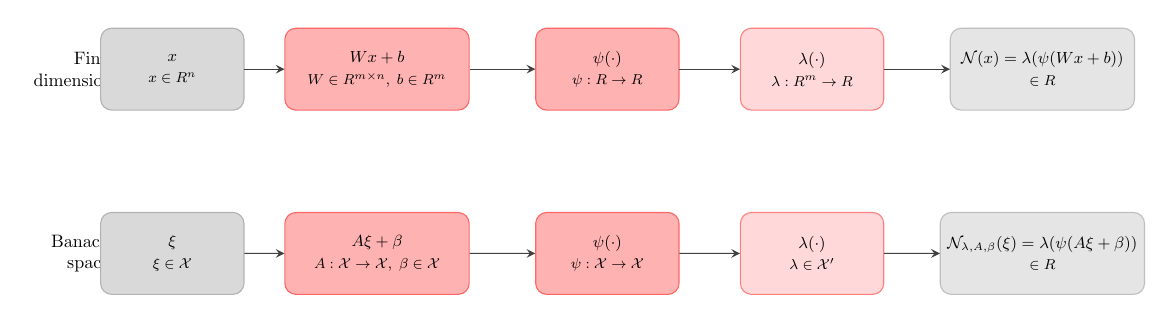
\begin{tikzpicture}[
    scale=0.65,
    transform shape,
    box/.style={rectangle, rounded corners=4pt, minimum width=28mm, minimum height=16mm, inner sep=4pt, align=center},
    >=stealth
]
\definecolor{darkgrey}{RGB}{90,90,90}

% ======================
% TOP ROW: Finite-dimensional
% ======================
\node[font=\normalsize, align=right] at (-1.8, 0.0)
    {Finite-\\dimensional};

% Input
\node[box, fill=gray!30, draw=gray!60] (FI) at (0, 0)
    {\small$x$\\\footnotesize$x \in \mathbb{R}^n$};

% Affine step
\node[box, fill=red!30, draw=red!60, minimum width=36mm] (FA) at (4, 0)
    {\small$Wx + b$\\\footnotesize$W \in \mathbb{R}^{m \times n},\; b \in \mathbb{R}^m$};

% Activation
\node[box, fill=red!30, draw=red!60] (FP) at (8.5, 0)
    {\small$\psi(\cdot)$\\\footnotesize$\psi : \mathbb{R} \to \mathbb{R}$};

% Linear functional
\node[box, fill=red!15, draw=red!50] (FL) at (12.5, 0)
    {\small$\lambda(\cdot)$\\\footnotesize$\lambda : \mathbb{R}^m \to \mathbb{R}$};

% Output
\node[box, fill=gray!20, draw=gray!50, minimum width=36mm] (FO) at (17.0, 0)
    {\small$\mathcal{N}(x) = \lambda(\psi(Wx+b))$\\\footnotesize$\in \mathbb{R}$};

% Arrows top row
\draw[->, draw=darkgray] (FI) -- (FA);
\draw[->, draw=darkgray] (FA) -- (FP);
\draw[->, draw=darkgray] (FP) -- (FL);
\draw[->, draw=darkgray] (FL) -- (FO);

% ======================
% BOTTOM ROW: Banach space
% ======================
\node[font=\normalsize, align=right] at (-1.8, -3.6)
    {Banach\\space};

% Input
\node[box, fill=gray!30, draw=gray!60] (BI) at (0, -3.6)
    {\small$\xi$\\\footnotesize$\xi \in \mathcal{X}$};

% Affine step
\node[box, fill=red!30, draw=red!60, minimum width=36mm] (BA) at (4, -3.6)
    {\small$A\xi + \beta$\\\footnotesize$A : \mathcal{X} \to \mathcal{X},\; \beta \in \mathcal{X}$};

% Activation
\node[box, fill=red!30, draw=red!60] (BP) at (8.5, -3.6)
    {\small$\psi(\cdot)$\\\footnotesize$\psi : \mathcal{X} \to \mathcal{X}$};

% Linear functional
\node[box, fill=red!15, draw=red!50] (BL) at (12.5, -3.6)
    {\small$\lambda(\cdot)$\\\footnotesize$\lambda \in \mathcal{X}'$};

% Output
\node[box, fill=gray!20, draw=gray!50, minimum width=36mm] (BO) at (17.0, -3.6)
    {\small$\mathcal{N}_{\lambda,A,\beta}(\xi) = \lambda(\psi(A\xi+\beta))$\\\footnotesize$\in \mathbb{R}$};

% Arrows bottom row
\draw[->, draw=darkgray] (BI) -- (BA);
\draw[->, draw=darkgray] (BA) -- (BP);
\draw[->, draw=darkgray] (BP) -- (BL);
\draw[->, draw=darkgray] (BL) -- (BO);

\end{tikzpicture}
\caption{Correspondence between the finite-dimensional neuron
$\mathcal{N}(x) = \lambda(\psi(Wx+b))$ and its infinite-dimensional
analogue $\mathcal{N}_{\lambda,A,\beta}(\xi) = \lambda(\psi(A\xi+\beta))$
on a Banach space $\mathcal{X}$. Each ingredient in the finite-dimensional
setting has a direct Banach-space counterpart: the matrix $W$ becomes a
bounded linear operator $A:\mathcal{X}\to\mathcal{X}$, the bias $b$
becomes an element $\beta\in\mathcal{X}$, and the linear functional
$\lambda:\mathbb{R}^m\to\mathbb{R}$ becomes a continuous linear
functional $\lambda\in\mathcal{X}'$.}
\label{fig:neuron_analogy}
\end{figure}


Let now $\xi \in \mathcal{X}$, where $\mathcal{X}$ is a Banach space. The finite-dimensional quantities in \eqref{eq:finite_neuron_op} must then be replaced by objects that act on elements of the Banach space rather than on finite-dimensional vectors.

\begin{description}
    \item[Linear transformation and bias.]
    The matrix $W$ is replaced by a bounded linear operator
    $A : \mathcal{X} \to \mathcal{X}$, and the bias vector $b$
    by a bias element $\beta \in \mathcal{X}$. Thus the affine
    step becomes
    \[
        \xi \mapsto A\xi + \beta.
    \]

    \item[Activation function.]
    In finite dimensions, $\psi$ acts coordinate-wise on a vector.
    In the Banach-space setting, we instead require an activation
    map $\psi : \mathcal{X} \to \mathcal{X}$. Following
    \citet{Benth2024}, one possible construction is
    \begin{equation}
        \psi(\xi)
        =
        \sum_{j=1}^\infty
        \tilde{\psi}_j\bigl(\rho(\xi)\bigr)\,\zeta_j,
    \label{eq:inf_activation}
    \end{equation}
    where $\rho \in \mathcal{X}'$ is a continuous linear
    functional, each $\tilde{\psi}_j : \mathbb{R} \to \mathbb{R}$
    is a classical sigmoidal function, and
    $\zeta_j \in \mathcal{X}$. The input is an element of $\mathcal{X}$, and the output is again an element of $\mathcal{X}$.

    \item[Scalar output map.]
    In finite dimensions, the final scalar output is obtained by
    a linear map $\mathbb{R}^m \to \mathbb{R}$, represented by a
    row vector. In the Banach-space setting, the corresponding
    object is a continuous linear functional
    $\lambda \in \mathcal{X}'$. 
\end{description}

With these replacements, an infinite-dimensional neuron
\citep{Benth2024} takes the form
\begin{equation}
    \mathcal{N}_{\lambda, A, \beta}(\xi)
    =
    \lambda\bigl(\psi(A\xi + \beta)\bigr),
    \qquad \xi \in \mathcal{X}.
\label{eq:inf_neuron}
\end{equation}
It still produces a scalar output, but its input is now an element of the Banach space $\mathcal{X}$ rather than a vector in $\mathbb{R}^n$.

\subsection{Neural networks on Banach spaces}
 
A one-hidden-layer network of width $M$ is a linear superposition of $M$ neurons of the form \eqref{eq:inf_neuron}:
\begin{equation}
    \mathcal{N}(\xi)
    :=
    \sum_{j=1}^M
    \mathcal{N}_{\lambda_j, A_j, \beta_j}(\xi).
\label{eq:inf_network}
\end{equation}
To produce a $\mathcal{Y}$-valued output, one aggregates $p$ real-valued networks scaled by linearly independent unit vectors $\mu_1, \ldots, \mu_p \in \mathcal{Y}$:
\begin{equation}
    \mathcal{N}^p(\xi)
    =
    \sum_{i=1}^p \mathcal{N}^{(i)}(\xi)\,\mu_i.
\label{eq:inf_network_Y}
\end{equation}
Setting $\mathcal{X} = \mathbb{R}^n$, the operator $A_j$ reduces to a matrix, $\beta_j$ to a vector, and $\lambda_j$ to a row vector, recovering
\eqref{eq:finite_neuron_op}.

For the Universal Approximation Theorem to apply, the activation function $\psi$ must satisfy a \emph{separation property} \citep{Benth2024}: there exist $\varphi \in \mathcal{X}' \setminus \{0\}$ and limit values $\nu_+, \nu_-, \nu_0 \in \mathcal{X}$ such that
\begin{equation}
    \lim_{\alpha \to \infty} \psi(\alpha \xi)
    =
    \begin{cases}
        \nu_+ & \text{if } \varphi(\xi) > 0, \\
        \nu_- & \text{if } \varphi(\xi) < 0, \\
        \nu_0 & \text{if } \varphi(\xi) = 0,
    \end{cases}
\label{eq:separation}
\end{equation}
with $\nu_+$ or $\nu_-$ not in the span of the other two. This is the infinite-dimensional generalisation of the non-constancy condition in Theorem~\ref{thm:UAT}: the activation function must separate the space $\mathcal{X}$ into distinguishable regions. The construction \eqref{eq:inf_activation} satisfies this property provided the $\tilde{\psi}_j$ are classical sigmoidal functions and the $(\zeta_j)$ form a summable sequence in $\mathcal{X}$.

We now state the universal approximation theorem for networks on Banach spaces, following \citet{Benth2024}.

\begin{theorem}[Universal approximation theorem on Banach spaces, \citealt{Benth2024}]
\label{thm:UAT_inf}
Let $\psi : \mathcal{X} \to \mathcal{X}$ be continuous, bounded, and separating in the sense of \eqref{eq:separation}. Suppose $\mathcal{F} : \mathcal{X} \to \mathcal{Y}$ is a continuous operator. Then for any compact set $K \subset \mathcal{X}$ and any $\varepsilon > 0$, there exist $p \in \mathbb{N}$, linearly independent unit vectors $\mu_1, \ldots, \mu_p \in \mathcal{Y}$, and real-valued networks $\mathcal{N}^{(1)}, \ldots, \mathcal{N}^{(p)}$ of the form \eqref{eq:inf_network} such that
\[
    \sup_{\xi \in K}
    \bigl\|\mathcal{F}(\xi)
    - \mathcal{N}^p(\xi)\bigr\|_{\mathcal{Y}}
    < \varepsilon,
\]
where $\mathcal{N}^p$ is defined in \eqref{eq:inf_network_Y}.
\end{theorem}

The theorem guarantees that any continuous operator between Banach spaces can be approximated arbitrarily well on compact sets by a network of the form \eqref{eq:inf_network_Y}. It is therefore the Banach-space analogue of the finite-dimensional universal approximation result stated in Theorem~\ref{thm:UAT}. As in the finite-dimensional case, the theorem is an existence result: it does not specify how large the network must be, nor how the approximating parameters are to be found in practice. The critical assumption is continuity of the operator $\mathcal{F}$, and verifying this property is therefore the key step before the theorem can be applied.


% ----- PLACEHOLDER END -------